\section{Généralisation}
\subsection{Cas avec n communautés}
On peut a présent généraliser à un nombre de communautés $q \geq 2$.
Nous allons supposer que les communautés sont de même taille, à savoir $n_q = \frac{n}{q}$.
\paragraph{}\label{rq:contrainte model}
Une première contrainte apparaît, de par l'utilisation des théorèmes \ref{th:1} et \ref{th:2}, sur les valeurs des probabilités de la matrice d'adjacence $A$.
En effet, d'après le \autoref{th:1}, pour que la matrice $X$ est une mesure spectrale qui tende vers la loi de Wigner il faut que la norme 1 des vecteurs lignes de son profil de variance soient égales ($\parallel x \parallel_1 = \sum_{j=1}^{n}|x_j|$).
Par conséquent, si on veut augmenter le nombre de communautés $q$ dans le modèle, on est forcé de garder deux probabilités $p_{in}$ et $p_{out}$ qui jouent le même rôle que celles introduites précédemment (cf. \ref{rq:probability}).\\

On sait que la matrice d’adjacence du graphe sous le SBM à $q$ communautés est $A = X + \langle A \rangle$.  
Pour poursuivre l'analyse on va suivre la trame suivante:
\begin{itemize}
	\item[1-] Trouver l'équation de $\langle A \rangle$ ;
	\item[2-] Trouvez l'équation de X et déterminer son profil de variance ;
	\item[3-] Trouvez les $q$ valeurs propres associées aux perturbations de rang 1 ;
	\item[4-] Trouver $p_{lim}$.\\
\end{itemize}

% ------------------------------------------------- 1- trouver <A>  -------------------------------------------------
\subsubsection*{1- Équation de $\langle A \rangle$}
$\langle A \rangle$ étant symétrique, le théorème spectral nous dis qu'il existe une base orthonormée telle que $\langle A \rangle = \sum_{n}^{i=1}\lambda_i\mathbf{u}_i\mathbf{u}_i^{\star}$.
Après les calculs on trouve:
\begin{align} 
\langle A \rangle :&= n_q(p_{in} + (q-1)p_{out}) \mathbf{u}_1\mathbf{u}_1^{\star} + n_q(p_{in}-p_{out})\sum_{i=1}^{q-1}\mathbf{u}_i\mathbf{u}_i^{\star}\\
				   &= \frac{c_{in} + (q-1)c_{out}}{q} \mathbf{u}_1\mathbf{u}_1^{\star} + \frac{c_{in}-c_{out}}{q}\sum_{i=1}^{q-1}\mathbf{u}_i\mathbf{u}_i^{\star}
\end{align}\\
où les trois valeurs propres sont $0$, $n_q(p_{in} + (q-1)p_{out})$, $n_q(p_{in}-p_{out})$ de multiplicité $q(n_q - 1)$, $1$, $q-1$.\\

% ------------------------------------------------- 2- trouver X  -------------------------------------------------
\subsubsection*{2- Profil de variance de $\frac{X}{\sqrt{n}}$}
De la même manière que dans \autoref{ch:Analyse spectrale de la matrice d'adjacence} on trouve:
\begin{equation}
	X_{ij} \sim \left\{
	\begin{array}{lr}
		\sigma_{in} Z_{ij} & : (i,j \in P_{in}) \\
		\sigma_{out} Z_{ij} & : (i,j \in P_{out})
	\end{array}
\right.\nonumber
\end{equation}
Où $Z_{ij} = \frac{B_{ij}(p) - p}{\sqrt{p(1-p)}} \;\;avec \; p = p_{in} \lor p_{out}$, $B_{ij}(p) \sim B(p)$, $B(p)$ loi de Bernoulli de paramètre p\\
La somme de n'importe quel vecteur ligne (ou colonne) du profil de variance de $\frac{X}{\sqrt{n}}$ est égale à : 
\begin{align}
\label{eq:sigma2} 
\sigma^2 = \frac{\sigma_{in}^2 + (q-1)\sigma_{out}^2}{q}
\end{align}
Le profil de variance de $\frac{X}{\sqrt{n}}$ est donc une matrice bi-stochastique.\\
% ------------------------------------------------- 3- trouver les vp -------------------------------------------------
\subsubsection*{3- Valeurs propres de $\frac{A}{\sqrt{n}}$}
Soit $\lambda$ une valeur propre de $\frac{A}{\sqrt{n}}$ et le vecteur propre associé.
\begin{align}
&\Leftrightarrow \frac{A}{\sqrt{n}}v =\lambda v \nonumber \\
&\Leftrightarrow (\Gamma - \lambda I)v =-\alpha \mathbf{11}^Tv - \beta \sum_{i=1}^{q-1}\mathbf{u}_i\mathbf{u'}_i^T \label{eq:generalize}
\end{align}
Pour trouver la valeur propre associée à $\mathbf{u}_1$ on multiplie à gauche par $\mathbf{u}_1^{\star}(\Gamma -\lambda I)^{-1}$ et on obtient:
\begin{align}
\eqref{eq:generalize} &\Leftrightarrow \mathbf{u}_1^{\star}v =-\alpha \mathbf{u}_1^{\star}(\Gamma -\lambda I)^{-1}\mathbf{u}_1\mathbf{u}_1^{\star}v - \beta \mathbf{u}_1^{\star}(\Gamma -\lambda I)^{-1}\sum_{i=1}^{q-1}\mathbf{u}_i\mathbf{u}_i^{\star}v \nonumber\\
&\xrightarrow[n \to +\infty]{} 1 = -\alpha g_{wig}^{\sigma^2}(\lambda) \nonumber\\
&\Leftrightarrow 1 = \alpha \frac{\lambda + \sqrt{\lambda^2 - 4\sigma^2}}{2\sigma^2} \nonumber\\
&\Leftrightarrow \lambda = \frac{c_{in} + (q-1)c_{out}}{q\sqrt{n}} + \frac{q\sqrt{n}\sigma^2}{c_{in} + (q-1)c_{out}} \label{eq:z_2 generalize}
\end{align}
Si on remplace $q$ par $2$ on retrouve l'équation \eqref{z_2}.\\
Pour trouver les valeurs propres associée aux $\mathbf{u}_i, \; \forall i \in \{2, \cdots, q-1\}$ on multiplie à gauche par $\mathbf{u}_2^{\star}(\Gamma -\lambda I)^{-1}$ et on obtient:
\begin{align}
\eqref{eq:generalize} &\Leftrightarrow \mathbf{u}_2^{\star}v =-\alpha \mathbf{u}_2^{\star}(\Gamma -\lambda I)^{-1}\mathbf{u}_1\mathbf{u}_1^{\star}v - \beta \mathbf{u}_2^{\star}(\Gamma -\lambda I)^{-1}\sum_{i=1}^{q-1}\mathbf{u}_i\mathbf{u}_i^{\star}v \nonumber\\
&\xrightarrow[n \to +\infty]{} 1 = -\beta g_{wig}^{\sigma^2}(\lambda) \nonumber\\
&\Leftrightarrow 1 = \beta \frac{\lambda + \sqrt{\lambda^2 - 4\sigma^2}}{2\sigma^2} \nonumber\\
&\Leftrightarrow \lambda = \frac{c_{in} - c_{out}}{q\sqrt{n}} + \frac{q\sqrt{n}\sigma^2}{c_{in} - c_{out}}\label{eq:z_1 generalize}
\end{align}
Si on remplace $q$ par $2$ on retrouve l'équation \eqref{z_1}.\\
Les valeurs propres de $A$ pour les valeurs propres de $\langle A \rangle$ égales à zéros appartiennent au support de la distribution de Wigner.
Elles n'apportent donc aucune information supplémentaire sur la structure de communauté du graphe étudié.\\   

Nous noterons $z_1 =$ \eqref{eq:z_1 generalize}  et $z_2 =$ \eqref{eq:z_2 generalize} pour la suite.
 

% ------------------------------------------------- 4- trouver p_lim -------------------------------------------------
\subsubsection*{4- Seuil de décidabilité $p_{lim}$}
Nous cherchons maintenant à déterminer $p_{lim}$.
La condition limite naturelle est celle où la valeur propre $z_2$ qui sort du support de la distribution de Wigner est égale au bord droit du support de la mesure spectrale de la matrice A.
On a alors 
\begin{align*}
	&\Leftrightarrow \lambda^+ = z_1\\
	&\Leftrightarrow 2 \sigma = \frac{c_{in} - c_{out}}{q\sqrt{n}} + \frac{q\sqrt{n}\sigma^2}{c_{in} - c_{out}}\\
	&\Leftrightarrow 0 = \beta \sigma^2 - 2 \sigma + \alpha \\
	&\text{après résolution de l'équation on obtient une unique solution}\\
	&\Leftrightarrow p_{in} - p_{out} = \frac{q\sigma}{\sqrt{n}}  \\
\end{align*}
Donc
\begin{equation}
	p_{lim} = \frac{\sqrt{q(\sigma_{in}^2 + (q-1)\sigma_{out}^2)}}{\sqrt{n}} = \frac{q\sigma}{\sqrt{n}}  \\
\end{equation}


% ------------------------------------------------- 5- résumer -------------------------------------------------
\subsection{Bilan}
Ci-dessous le bilan de la généralisation:
\begin{align*}
	\sigma^2&: \frac{\sigma_{in}^2 + (q-1)\sigma_{out}^2}{q} \\
	z_1&: \frac{c_{in} - c_{out}}{q\sqrt{n}} + \frac{q\sqrt{n}\sigma^2}{c_{in} - c_{out}}\\
	z_2&: \frac{c_{in} + (q-1)c_{out}}{q\sqrt{n}} + \frac{q\sqrt{n}\sigma^2}{c_{in} + (q-1)c_{out}}\\
	p_{lim}&: \frac{\sqrt{q(\sigma_{in}^2 + (q-1)\sigma_{out}^2)}}{\sqrt{n}} \\
\end{align*}

% ------------------------------------------------- 6- Simulation -------------------------------------------------
\subsection{Simulations}
\begin{figure}[H]
\centering
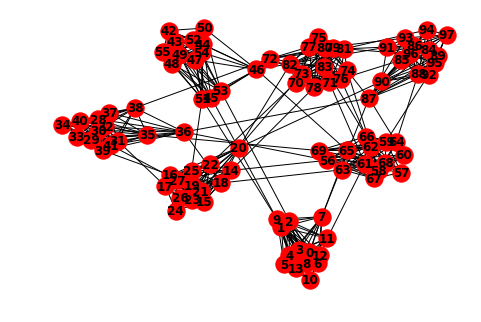
\includegraphics[scale=0.6]{static/graph_q7_n100_pin08_pout0011.png}
\caption{Graphe généré à partir des paramètres: $q=7$ $n=100$, $p_{in}=0.8$, $p_{out}=0.01$}
\end{figure}
\begin{figure}[H]
\centering
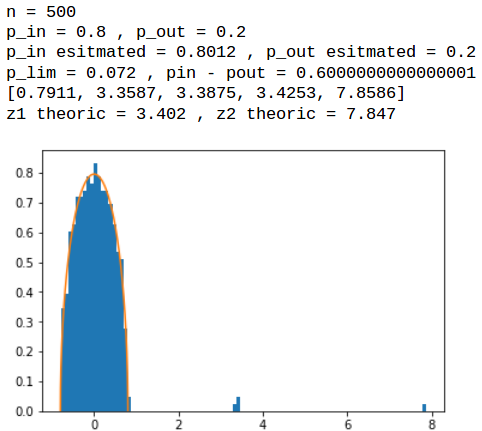
\includegraphics[scale=0.6]{static/spectral_q4_n500_pin08_pout02}
\caption{$q=4$, $n=500$, $\Delta p=0.6$}
\label{n500delta-05}
\end{figure}
\subsection{Limites du modèle}
Le première limite de ce modèle est que l'on est cantonné à des communautés de même taille $n_q$.
En effet si on change ce paramètre pour chacune des communautés alors le \autoref{th:1} n'est plus applicable, la somme des éléments de chaque vecteurs ligne du profil de variance n'est plus constant.\\

La deuxième contrainte est le fait que l'on doit toujours garder deux paramètres $p_{in}$ et $p_{out}$ indépendamment du nombre de communautés $n_q$ et du nombre de nœuds dans le graphe $n$.
Idéalement nous souhaiterions avoir un paramètre $p_{ij}$ correspondant à la probabilité d'avoir une arrête entre le nœud $i$ et le nœud $j$ et ce $\forall i<j$.\\
Une manière d'encoder ces paramètres est d'utiliser la relation suivante $p_{ij} = q_iq_jC_{\alpha}$
\begin{align}
	p_{ij} &= q_iq_jC_{g_ig_j}
\end{align}
Où $q_i$ est la probabilité intrinsèque du nœud $i$ à avoir une arrête, $g_i$ est la communauté correspondant au nœud $i$ et $C_{g_ig_j}$ est le facteur de correction par communauté.\\
Cette formalisation plus générale est très répandu dans la théorie de la détection de communauté spectrale.